\section{Discussion}

% Finding 1: SOT improves meta-learners but not non-meta learners
This study reveals that the SOT module significantly enhances the performance of all meta-learners on both datasets, but not of non-meta learners. The reason lies in their distinct training methodologies. Meta-learners undergo episodic training, mimicking a few-shot learning scenario with support and query samples from various classes. This approach allows the backbone and SOT module to jointly optimise, enhancing the matching between support and query samples. Conversely, non-meta learners are trained with random mini-batches from the entire training set, focusing on general multi-class classification without distinguishing between support and query samples. Consequently, their embeddings, though effective in standard classification tasks, do not transfer well to few-shot evaluations. This is illustrated in Figure~\ref{fig:sot-embeddings}: the SOT embeddings for a Prototypical Network show clear clustering of support and query samples from the same class, unlike those for the Baseline model.

% TODO: Adjust title of right subplot
\begin{figure}[h!]
    \centering
    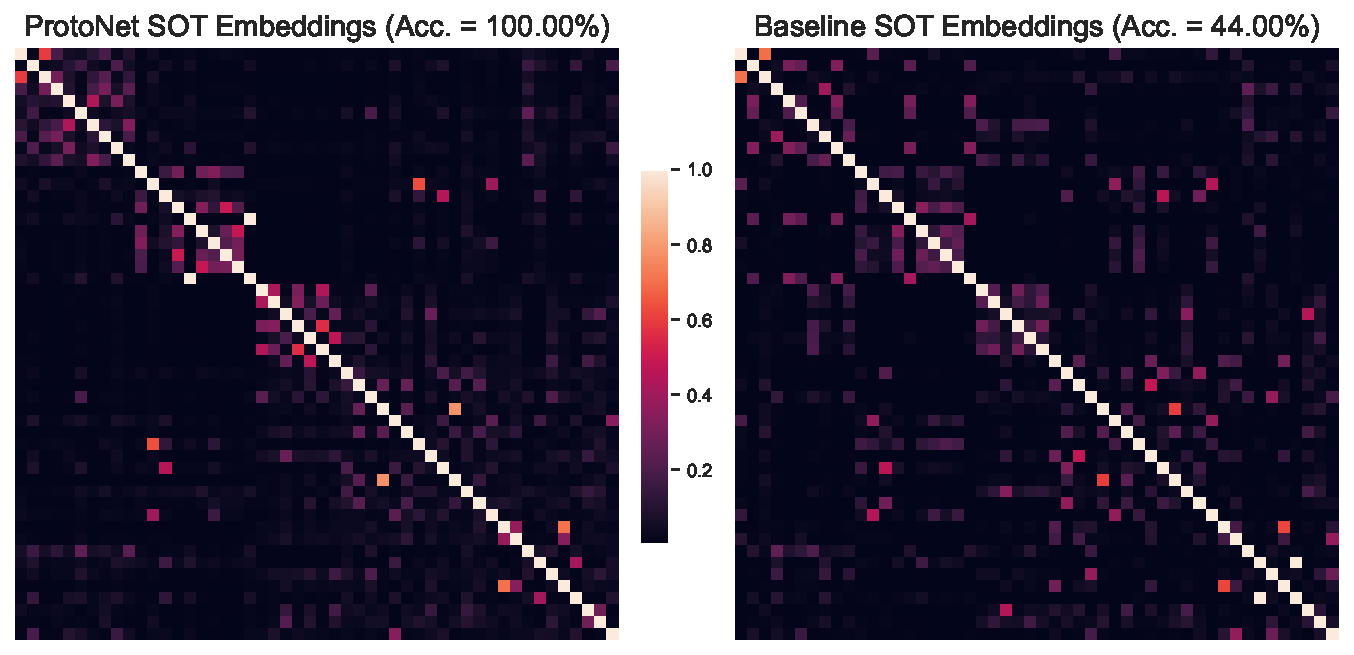
\includegraphics[width=1\columnwidth]{../figures/sot-embeddings.pdf}
    \caption{SOT Embeddings for Prototypical Network (left) and Baseline (right) on the SwissProt dataset for a random episode from the meta-test split for a 5-way-5-shot task with 5 query samples. Support and query samples from the same class are adjacent.}
    \label{fig:sot-embeddings}
\end{figure}

% Finding 2: SOT results in almost perfect performance even in most difficult few-shot learning setting
The SOT module also improves the performance of meta-learners in the most challenging few-shot learning setting, i.e. 10-way-1-shot. This indicates that the SOT module is capable of learning a highly effective embedding, even with a single support sample per class. We hypothesise that with a more challenging dataset or even higher number of ways, the performance would decrease. However, given the limitations of the datasets, we were unable to test this hypothesis.

% Finding 3: SOT improves performance in interaction with LSTM re-embedding
While studying the interaction of the SOT module with the LSTM re-embeddings of support and query samples in Matching Networks an interesting observation was made. 

we observed that the SOT module enhances the performance of the LSTM re-embedding, but not vice versa. This is likely due to the fact that the LSTM re-embedding is a more powerful embedding than the SOT module, and thus the SOT module is unable to improve it further. Conversely, the SOT module is able to enhance the performance of the baseline embedding, as it is less powerful.
% Why? :(